\documentclass[a4paper,12pt]{article}
\usepackage[utf8]{inputenc}
\usepackage[german, ngerman]{babel}
\usepackage{graphicx}
\usepackage[figurename=Bild]{caption}
\usepackage{inputenc}
\usepackage{geometry}


%opening
\title{Recherche der Provider und Partner}
\author{Burak Erol}

\begin{document}

\section{Recherche der Partner und Provider}

Die Recherche zeigt auf zwei verschiedenen Excel-Dokumenten eine Liste aller Partner und Provider die f�r die Suchabfragen des Browsers kontaktiert werden. Es wird aufgelistet was die Webseite Inhaltlich spiegelt. Die Dokumente sollen eine �bersicht dieser Seiten f�r die Suchabfragen zeigen. Die Webseiten unterscheiden sich im Kontext, denn es befinden sich sowohl wissenschaftliche, technische, kulturelle als auch Personen spezifische Inhalte auf diesen verschiedenen Providern.

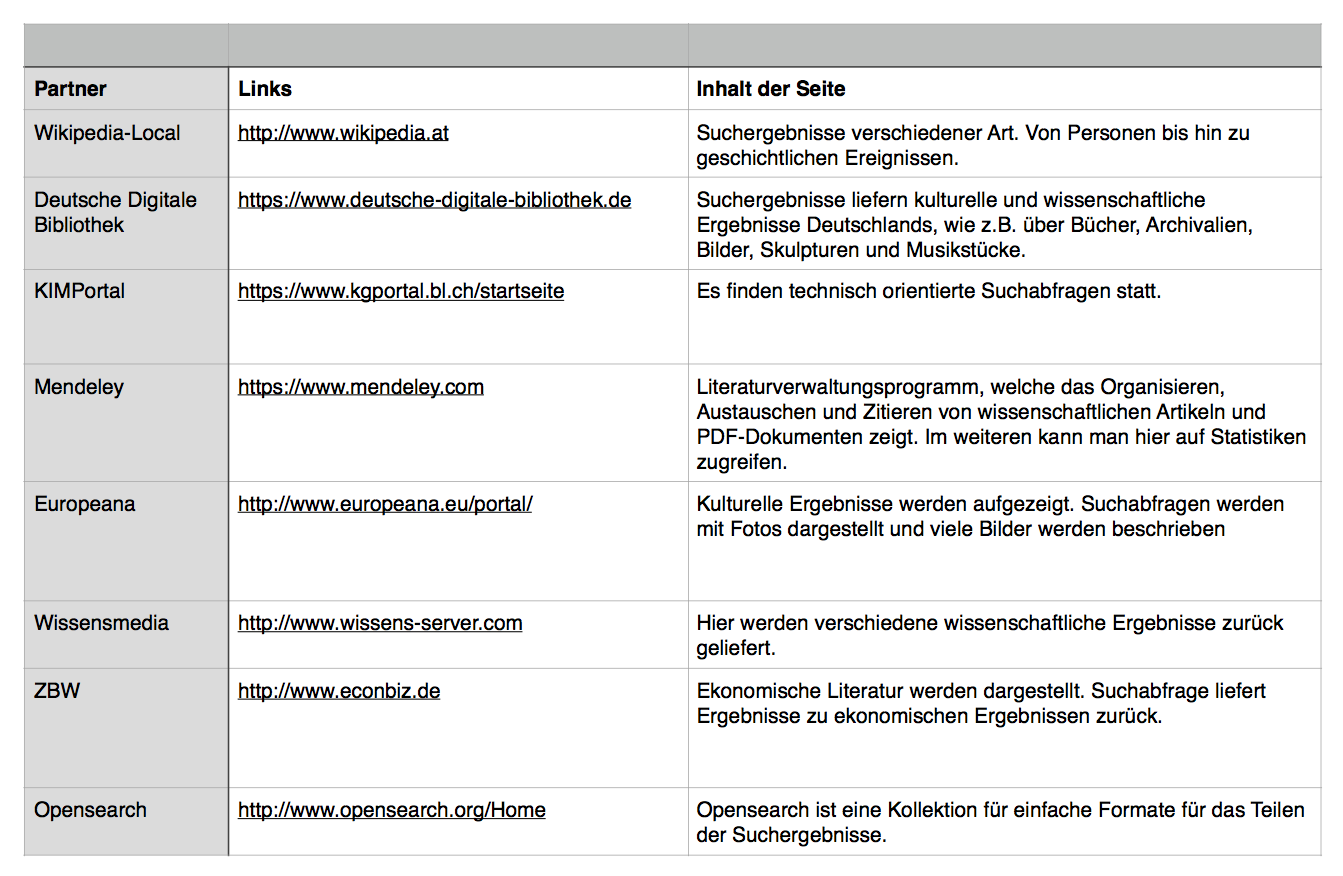
\includegraphics[width=12cm]{Pics/PartnerList}
\newpage
\includegraphics[width=12cm]{Pics/Provider}

\end{document}
